\documentclass[11pt]{article}
\usepackage[margin=1in]{geometry}
\usepackage{amsmath,amssymb}
\usepackage{xcolor}
\usepackage{setspace}
\usepackage{float}
\usepackage[hidelinks]{hyperref}
\usepackage{booktabs}
\usepackage{graphicx}
\usepackage{enumitem}
\usepackage{subcaption}
\usepackage{multirow}
\setlength{\parskip}{6pt}
\setlength{\parindent}{0pt}
\allowdisplaybreaks[3]

\newcommand{\reviewer}[1]{\vspace{0.4em}\noindent\textbf{Reviewer comment.} #1}
\newcommand{\response}[1]{\vspace{0.2em}\noindent\textbf{Response.} #1}
\newcommand{\revise}[1]{\vspace{0.2em}\noindent\textbf{Revision made.} #1}
\newcommand{\red}[1]{\textcolor{red}{#1}}

\title{\textbf{Response to the Referee Report for Manuscript IP-105150.R1}}
\author{}
\date{}

\begin{document}
\maketitle

Dear Editor and Referee,

We sincerely thank the referee for the careful reading of our revised manuscript and for the detailed comments. We agree that the previous revision did not explain sufficiently how the proposed morphology detection procedure is connected to the actual MA-RFM experiments.
In this revision, we have made the role of the shape-detection step explicit, added implementation details, and corrected all minor issues listed in the report.

In addition to the specific points raised by the reviewers, we would like to emphasize more clearly the role of the former Algorithm 3, now renumbered as Algorithm 2 in the revised manuscript. For clarity, in what follows we refer to it uniformly as Algorithm 2. Its essential purpose is to serve as the bridge between the first stage, namely IA-RFM, and the second stage, namely the morphology-aware basis enhancement. Starting from the coarse IA-RFM reconstruction $S^{(0)}$, the algorithm performs clustering and morphological post-processing on the detected active region, extracts posterior shape parameters, and then uses shape-dependent thresholds to determine which type of morphology-aware basis functions should be added in the second stage.

The referee's concern is therefore whether the second stage uses prior information in a way that would amount to assuming access to the true geometry. We agree that this concern is entirely reasonable, and that our previous manuscript did not explain this point clearly enough.
What is prescribed a priori in our implementation is not the exact geometry of the unknown source, but only an admissible collection of morphology classes for the enrichment space. This candidate library is not meant to be an immutable object: it is a solver-design choice that may depend on the problem family, and it may be extended when the stage-one coarse reconstruction exhibits stable evidence of an additional regular morphology. 
Such an extension operates only at the level of admissible basis families, not at the level of ground-truth geometric parameters. The role of the detection algorithm is then to determine, from the coarse reconstruction and the corresponding shape indicators, which candidate family should be activated and which geometric parameters should be passed to the second stage. 
In particular, the centers, radii, widths, and related shape parameters used in the enriched basis are inferred from the coarse reconstruction through the detection algorithm, rather than taken from the exact source. To make this point fully transparent and reproducible, we have also chosen to make the code publicly available.

Accordingly, we have implemented several significant improvements in the revised manuscript:
\begin{enumerate}
    \item We simplify Algorithm 2 in the revised manuscript. In particular, we remove the unnecessary threshold parameters $t_{\text{AR}}$, $t_{\Sigma}$, and $t_p$, and introduce a unified regular-shape threshold $t_{\text{reg}}$. The circle case is now included as a special case of the more general ellipsoid class, and the previous general-shape criteria are replaced by the new $t_{\text{reg}}$-based rule. Accordingly, we rerun the code for the numerical examples related to shape detection, update the corresponding detected geometric parameters and shape-classification results, and revise Table~9 consistently.
    \begin{table}[H]
      \centering
      \caption{Extracted geometric parameters and statistical indicators with $\delta=5\%$ by Algorithm
  3.}
      \label{tab:extracted_parameters}
      \resizebox{\textwidth}{!}{%
      \begin{tabular}{ccccccccc}
          \toprule
          {\emph{Ex}} & Cluster $k$ & $\boldsymbol{c}_k$ & $\boldsymbol{L}_k$ &
          $\mathcal{E}_{\text{rect}}^{(k)}$ & $\mathcal{E}_{\text{ellip}}^{(k)}$ &
          $\mathcal{E}_{\text{torus}}^{(k)}$ & $\mathcal{T}_k$ & $\sigma_k$ \\
          \midrule

          Ex 4.3 & 1 & (5.00e-01, 5.00e-01) & (2.03e-01, 2.03e-01) & 0.0885 &
  \textbf{0.0138} & - & \textbf{Ellipsoid} & Sigmoid \\
          \midrule

          \multirow{2}{*}{Ex 4.4}
            & 1 & (-6.06e-02, 1.24e-04) & (6.40e-02, 6.60e-02) & 0.0789 & \textbf{0.0379}
  & - & \textbf{Ellipsoid} & Exp \\
            & 2 & (8.04e-02, 9.14e-06) & (6.40e-02, 6.60e-02) & 0.0801 & \textbf{0.0364}
  & - & \textbf{Ellipsoid} & Exp \\
          \midrule

          \multirow{2}{*}{Ex 4.5}
            & 1 & (3.90e-01, 5.01e-01) & (1.10e-01, 2.05e-01) & \textbf{0.0304} & 0.1284
  & - & \textbf{Rectangle} & Sigmoid \\
            & 2 & (7.11e-01, 5.00e-01) & (2.02e-01, 2.05e-01) & 0.0922 & \textbf{0.0108}
  & - & \textbf{Ellipsoid} & Sigmoid \\
          \midrule

          Ex 4.6 & 1 & (6.01e-01, 2.51e-01) & - & 0.0698 & 0.0613 & - & \textbf{general} & Sigmoid \\
          \midrule

          \multirow{4}{*}{Ex 4.7}
            & 1 & (2.12e-01, 7.13e-01) & - & 0.1113 & 0.0675 & - & \textbf{general} & Sigmoid \\
            & 2 & (4.20e-01, 4.49e-01) & - & 0.1938 & 0.1211 & - & \textbf{general} & Sigmoid \\
            & 3 & (7.49e-01, 3.59e-01) & - & 0.1823 & 0.1102 & - & \textbf{general} & Sigmoid \\
            & 4 & (7.96e-01, 7.89e-01) & - & 0.2065 & 0.2152 & - & \textbf{general} & Sigmoid \\
          \midrule

          \multirow{2}{*}{Ex 4.8}
            & 1 & (3.01e-01, 4.99e-01, 3.00e-01) & (2.00e-01, 2.05e-01, 2.05e-01) &
  0.1737 & \textbf{0.0347} & 0.5461 & \textbf{Ellipsoid} & Exp/ReLU \\
            & 2 & (5.00e-01, 4.99e-01, 8.01e-01) & (2.05e-01, 2.05e-01, 2.05e-01) &
  0.1714 & \textbf{0.0340} & 0.5487 & \textbf{Ellipsoid} & Exp/ReLU \\
          \midrule

     Ex 4.9 & 1 &
      (-6.73e-05, -2.68e-03, 1.53e-03) &
      \begin{tabular}{@{}c@{}}
      $r_{1}$=1.49e-01 \\
      $R_{1}$=2.54e-01\\
      \end{tabular} &
      0.2854 & 0.1702 & \textbf{0.0402} & \emph{Tori} & Sigmoid \\
      \bottomrule
      \end{tabular}
      }
  \end{table}

    \item We introduce the residual indicator $\mathcal{E}_{\text{tori}}$ to improve the identification of doubly connected structures, especially in the three-dimensional setting.
    \item We add a new, more general numerical experiment in Example~4.7, where both the geometry and the functional form are unknown \emph{a priori} and the source consists of multiple irregular disjoint components. This example is included to demonstrate more clearly how Algorithm~2 drives the second-stage basis selection for irregular geometries.
\end{enumerate}

Below we provide a point-by-point response. Page, equation, table, and figure numbers refer to the revised manuscript.

\section*{Response to the Main Concern}

\reviewer{Algorithm 3 relies on geometric descriptors computed from an imprecise point
cloud extracted from the coarse solution, combined with several manually cho-
sen thresholds. The reliability of this procedure is inherently uncertain due
to: (i) the imprecision of the coarse solution from which the point cloud is
derived; }

\response{We thank the referee for this important comment. We agree that the reliability of the coarse first-stage reconstruction is crucial.
 This is precisely why, in the first stage, we adopt an adaptive integration strategy that places more sampling points in regions where both the reconstruction magnitude and the gradient magnitude are large. 
 In our numerical examples, the resulting final integration mesh $C_{\text{final}}$ is well aligned with these high-activity regions and is therefore able to capture the source's coarse geometric features. 
 Moreover, when passing from the first stage to the morphology-aware second stage, we do not use the detected geometric quantities in a rigid manner.
  Instead, we introduce perturbation tolerances such as $\epsilon_r$ and $\epsilon_c$ to account for the estimated geometric parameters, thereby accounting for possible inaccuracies in the detection step and improving the robustness of the enriched basis set.}

\reviewer{(ii) the fact that computing discrete curvature requires an ordered
boundary point sequence, yet the point cloud obtained by thresholding the
gradient field is unordered — the paper provides no explanation of how this
ordering is achieved;}

\response{We thank the referee for pointing this out. 
In the earlier implementation, the ordered boundary sequence in two dimensions was obtained by OpenCV contour extraction via \texttt{cv2.findContours}. However, your comment made us realize that this curvature-based classification logic was not sufficiently transparent and, in the revised algorithm, is not actually necessary. 
We have removed the curvature-related thresholds $t_{\Sigma}$ and $t_p$ and replaced them with a unified regular-shape threshold $t_{\text{reg}}$.
 In the revised criterion, if both $\mathcal{E}_{\text{ellip}}$ and $\mathcal{E}_{\text{rec}}$ are below $t_{\text{reg}}$, the cluster is classified as \emph{general};
  otherwise, it is assigned to the corresponding regular-shape branch. In the manuscript, we set $t_{\text{reg}}=0.05$ and include a sensitivity analysis for this choice. As a result, the revised shape-classification step no longer depends on discrete curvature and therefore no longer requires an ordered boundary point sequence.}

\reviewer{(iii) the absence of any theoretical justification or systematic sensitivity analysis for the chosen threshold values.}

\response{We thank the referee for this helpful suggestion. For the revised thresholds $t_{\text{reg}}$ and $t_{CV}$, we provide the following explanations:
\begin{enumerate}
    \item The threshold $t_{\text{reg}}$ is used to distinguish the regular-shape branch from the general-shape branch. In the revised manuscript, we set $t_{\text{reg}}=0.05$.
    \item To characterize the flatness of the reconstructed source profile, we use the coefficient-of-variation-type indicator
    \[
    CV_{\alpha}=\frac{\sigma(S_{\text{num}}^{\alpha})}{\mu(|S_{\text{num}}^{\alpha}|)}.
    \]
    The threshold $t_{CV}=0.7$ is then used to determine the activation profile in the second-stage enrichment: if $CV_{\alpha}<t_{CV}$, we use a sigmoid-type basis to represent a relatively smooth support profile; otherwise, we use more peak-type basis functions, such as those associated with \texttt{exp} or \texttt{ReLU}.
\end{enumerate}
To support these choices, we add a sensitivity analysis based on Example 4.5 with noise level $\delta=5\%$, $M_{\text{total}}=3200$. In this test, we keep the stage-one coarse reconstruction and the associated adaptive integration mesh fixed, and vary the two thresholds on the $3\times 3$ grid
\[
t_{\text{reg}}\in\{0.04,0.05,0.06\}, \qquad t_{CV}\in\{0.56,0.70,0.84\},
\]
which corresponds to applying a $20\%$ perturbation around the reference values $t_{\text{reg}}=0.05$ and $t_{CV}=0.70$. For each threshold pair, we rerun the shape-detection step, rebuild the corresponding morphology-aware enrichment, and solve the second-stage inverse problem with the same noisy data as in Example 4.5. 
\begin{figure}[H]
    \centering
    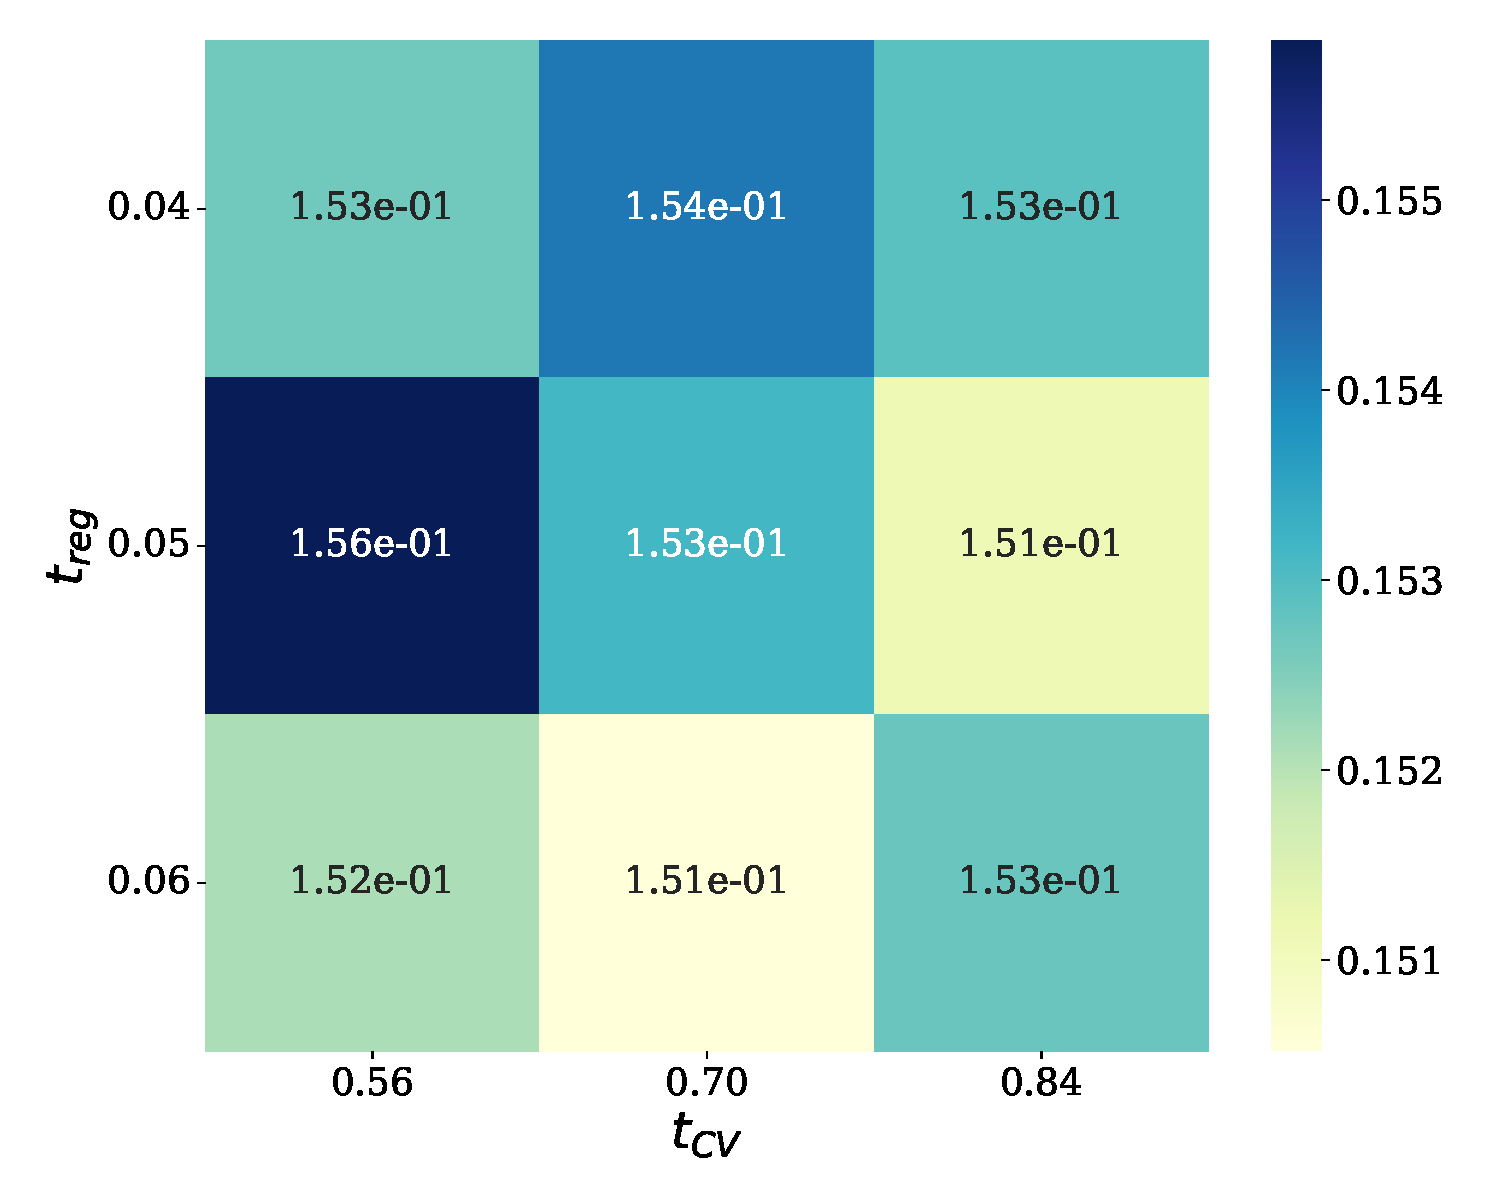
\includegraphics[width=0.5\textwidth]{shape_threshold_sensitivity.pdf}
    \caption{Sensitivity analysis for the shape-classification threshold $t_{\text{reg}}$ and the basis-profile-selection threshold $t_{CV}$, based on Example 4.5 with noise level $\delta=5\%$ and $M_{\text{total}}=3200$. The detected cluster patterns, morphology labels, and basis-profile choices remain stable under moderate perturbations of these thresholds. }
    \label{fig:shape-threshold-sensitivity}
\end{figure}


\begin{table}[H]
    \centering
    \caption{Detailed threshold-sensitivity results for Example 4.5 with noise level $\delta=5\%$.}
    \label{tab:shape-threshold-sensitivity}
    \small
    \resizebox{0.92\textwidth}{!}{%
    \begin{tabular}{cccp{0.2\textwidth}ccc}
        \toprule
        $t_{\text{reg}}$ & $t_{CV}$ & Clusters & \multicolumn{1}{c}{$\mathcal{T}_k$} & $\sigma_k$ & $\lambda_{\text{reg}}^2$ & $E_{l^2}(S_{\text{final}})$ \\
        \midrule
        0.04 & 0.56 & 2 & Ellipsoid, Rectangle & sigmoid & 1.00e-04 & 1.53e-01 \\
        0.04 & 0.70 & 2 & Ellipsoid, Rectangle & sigmoid & 1.00e-04 & 1.54e-01 \\
        0.04 & 0.84 & 2 & Ellipsoid, Rectangle & sigmoid & 1.00e-04 & 1.53e-01 \\
        0.05 & 0.56 & 2 & Ellipsoid, Rectangle & sigmoid & 1.00e-04 & 1.56e-01 \\
        0.05 & 0.70 & 2 & Ellipsoid, Rectangle & sigmoid & 1.00e-04 & 1.53e-01 \\
        0.05 & 0.84 & 2 & Ellipsoid, Rectangle & sigmoid & 1.00e-04 & 1.51e-01 \\
        0.06 & 0.56 & 2 & Ellipsoid, Rectangle & sigmoid & 1.00e-04 & 1.52e-01 \\
        0.06 & 0.70 & 2 & Ellipsoid, Rectangle & sigmoid & 1.00e-04 & 1.51e-01 \\
        0.06 & 0.84 & 2 & Ellipsoid, Rectangle & sigmoid & 1.00e-04 & 1.53e-01 \\
        \bottomrule
    \end{tabular}
    }
\end{table}
Figure \ref{fig:shape-threshold-sensitivity} and Table \ref{tab:shape-threshold-sensitivity} show that the algorithm consistently detects two clusters with the same morphology labels, namely \emph{Rectangle} and \emph{Ellipsoid}, and selects the \emph{Sigmoid} activation profile for both components. The selected regularization parameter remains unchanged, and the relative $L^2$ reconstruction error varies only mildly across the tested threshold range.
Consequently, we adopt the unified settings $t_{\text{reg}}=0.05$ and $t_{CV}=0.70$ in the reported numerical examples.}

\reviewer{More critically, in Examples 4.3–4.7, the basis functions used in MA-RFM are
all directly specified as hyperparameter settings, with no indication that they
were determined by Algorithm 3. From the presentation, it appears that the
basis function types, the number of source regions, and the functional form of
the source were all prescribed using prior knowledge of the true source, rather
than being automatically inferred from the coarse solution. This significantly
undermines the claim that MA-RFM can "adaptively identify critical regions
and incorporate morphology-aware activation functions." The superiority of MA-RFM under conditions where such prior knowledge is unavailable has not
been demonstrated.}

\response{We understand the referee's concern, and we agree that this part was not explained clearly enough in the previous version. The key point is that, before entering the second stage, all shape-related quantities are inferred from the stage-one coarse reconstruction by Algorithm~2. In particular, the morphology-aware basis family activated in the second stage is determined through this detection process, rather than prescribed from the true source geometry. The overall workflow is
\[
S^{(0)}_{M}\;\longrightarrow\; \mathcal{Q}\;\longrightarrow\; \{C_{\alpha}\}_{\alpha=1}^{K}\;\longrightarrow\; (\mathcal{T}_{\alpha},\theta_{\alpha},\sigma_{\alpha})\;\longrightarrow\;\mathcal{B}_{\rm new},
\]
where the coarse reconstruction is first converted into a candidate point cloud, then partitioned into clusters, and finally translated into morphology labels, geometric parameters, and basis-profile choices for the enriched space.

After obtaining the point cloud $\mathcal{Q}$, the procedure is as follows:
\begin{enumerate}
    \item \textit{Cluster Detection}: The number of sources $K$ is detected by DBSCAN. More precisely, Algorithm 2 partitions the candidate point set $\mathcal{Q}$ into $K$ disjoint clusters by the DBSCAN algorithm, using the adaptive neighborhood radius
    \[
  \varepsilon_{\rm clu}=c_\varepsilon h,\qquad
  h=\max_i(\Delta x_i),
  \]
  together with the minimum core-point size $N_{\min}^{\rm clu}$. These clusters are interpreted as the support regions of the detected sources:
    \[
    \mathcal{Q}=\bigcup_{\alpha=1}^{K} C_\alpha,\qquad
    C_i\cap C_j=\emptyset,\quad i\neq j.
    \]
    In our experiments, we use $c_\varepsilon=5$ and $N_{\min}^{\rm clu}=20$, and we further discard very small clusters as noise. To support this choice, we also performed a sensitivity analysis for the DBSCAN clustering parameters in Example 4.5 at noise level $\delta=5\%$, while keeping the same stage-one coarse reconstruction fixed. In that test, we varied the adaptive radius factor and the minimum core-point size on the grid
    \[
    c_{\varepsilon}\in\{4,5,6\}, \qquad N_{\min}^{\rm clu}\in\{16,20,24\},
    \]
    corresponding to a $20\%$ perturbation around the reference values $c_{\varepsilon}=5$ and $N_{\min}^{\rm clu}=20$. The detailed results are summarized in Table~\ref{tab:cluster-parameter-sensitivity}. Across all nine cases, the algorithm consistently detects two clusters, assigns the same morphology labels \emph{Rectangle} and \emph{Ellipsoid}, selects the same \emph{Sigmoid} activation profile, and yields only mild variation in the final relative $L^2$ reconstruction error.

\begin{table}[H]
    \centering
    \caption{Detailed clustering-parameter sensitivity results for Example 4.5 with noise level $\delta=5\%$.}
    \label{tab:cluster-parameter-sensitivity}
    \small
    \resizebox{0.92\textwidth}{!}{%
    \begin{tabular}{cccp{0.2\textwidth}ccc}
        \toprule
        $c_{\varepsilon}$ & $N_{\min}^{\rm clu}$ & Clusters & \multicolumn{1}{c}{$\mathcal{T}_k$} & $\sigma_k$ & $\lambda_{\text{reg}}^2$ & $E_{l^2}(S_{\text{final}})$ \\
        \midrule
        4.0 & 16 & 2 & Ellipsoid, Rectangle & sigmoid & 1.00e-04 & 1.54e-01 \\
        4.0 & 20 & 2 & Ellipsoid, Rectangle & sigmoid & 1.00e-04 & 1.54e-01 \\
        4.0 & 24 & 2 & Ellipsoid, Rectangle & sigmoid & 1.00e-04 & 1.53e-01 \\
        5.0 & 16 & 2 & Ellipsoid, Rectangle & sigmoid & 1.00e-04 & 1.55e-01 \\
        5.0 & 20 & 2 & Ellipsoid, Rectangle & sigmoid & 1.00e-04 & 1.51e-01 \\
        5.0 & 24 & 2 & Ellipsoid, Rectangle & sigmoid & 1.00e-04 & 1.52e-01 \\
        6.0 & 16 & 2 & Ellipsoid, Rectangle & sigmoid & 1.00e-04 & 1.54e-01 \\
        6.0 & 20 & 2 & Ellipsoid, Rectangle & sigmoid & 1.00e-04 & 1.55e-01 \\
        6.0 & 24 & 2 & Ellipsoid, Rectangle & sigmoid & 1.00e-04 & 1.53e-01 \\
        \bottomrule
    \end{tabular}
    }
\end{table}
    \item \textit{Shape Classification}: After clustering, each cluster is represented by a point cloud. 
    In two dimensions, the cluster points are rasterized to a binary image, processed by a morphological closing followed by one dilation, and then converted back to a detected outer boundary by \texttt{cv2.findContours}. 
    In three dimensions, the cluster points are voxelized and processed by binary closing, dilation, and erosion, and the boundary voxels are extracted as the XOR between the dilated and eroded occupancy grids.
     Based on the resulting boundary representation, the algorithm computes fitting residuals and radial descriptors, and classifies the cluster as \emph{Rectangle}, \emph{Ellipsoid}, \emph{Donut} when the annular/toroidal branch is detected, 
     or \emph{general}. It then outputs the corresponding parameters, such as the center $\boldsymbol{c}_\alpha$ and the length-scale parameters $\boldsymbol{L}_\alpha$ (or the major/minor radius for the donut branch).
    \item \textit{Basis Selection}: For each cluster, the activation profile $\sigma_\alpha$ is determined by the indicator $CV_\alpha$, which reflects the flatness of the reconstructed source values inside the cluster and then decides whether the second stage should use a peak-type basis(Exp or ReLU) or a flat-top basis(Sigmoid).
    \item \textit{Basis Assembly}: After the shape label $\mathcal{T}_\alpha$ and the activation profile $\sigma_\alpha$ are determined, the morphology-aware basis functions are generated accordingly. For regular clusters, i.e. \emph{Rectangle}, \emph{Ellipsoid}, or \emph{Donut}, we use analytic geometry-adapted basis functions of the form
    \[
    \phi_\alpha^{(j)}(\boldsymbol{x};K_\alpha^{(j)},\boldsymbol{\theta}_\alpha^{(j)})
    =
    \sigma_\alpha\!\left(K_\alpha^{(j)}\, d_{\mathcal{T}_\alpha}^{(j)}(\boldsymbol{x};\boldsymbol{\theta}_\alpha^{(j)})\right),
    \]
    where the shape parameters are sampled in a small neighborhood of the detected estimates in order to account for the uncertainty of the coarse reconstruction.
     For \emph{general} clusters, we first construct a numerical boundary $\hat{\Gamma}_\alpha$ from the detected point cloud and use it to define a numerical signed-distance-type branch. The additional local enhancement is then placed near the detected interface: 
     the centers of the local circular basis functions are sampled on a shrunken boundary generated from $\hat{\Gamma}_\alpha$, while their radii are determined by the mesh scale $h$.
     $$
\phi^{(j)}_{\mathrm{circular}}(\boldsymbol{x};K^{(j)},\boldsymbol{\theta}^{(j)})
=\mathrm{sigmoid}\!\left(
K^{(j)}\cdot\left((r^{(j)})^2-\|\boldsymbol{x}-\boldsymbol{c}^{(j)}\|_2^2\right)
\right), \quad j=1,\cdots,M_{\mathrm{circular}}.
$$
\end{enumerate}
In summary, the shape parameters used in the second stage are indeed inferred by Algorithm 2 from the coarse reconstruction, rather than taken directly from the ground truth. We have also implemented this complete workflow in the released code and made the code publicly available so that readers can fully reproduce our results.
}

\reviewer{While Table 9 in Appendix D.3 lists some geometric parameters and basis type classifications produced by Algorithm 3 for Examples
4.3–4.7, it is presented without any explanation and is not referenced anywhere
in the main text. Furthermore, it is not connected to the experimental setups
in Examples 4.3–4.7, making it impossible to verify whether Algorithm 3 was
actually used to drive basis function selection in these experiments.}

\response{We thank the referee for this important observation. In the previous version, Table~9 was indeed not sufficiently explained or linked to the main text. In the revised manuscript, we add explicit references to Table~9 in Examples 4.3--4.7 and clarify in the relevant hyperparameter-setting paragraphs that some of the shape parameters and basis-function types used in the second stage are selected according to the outputs of Algorithm~2, namely the detected morphology label and basis profile. We also add short references in the subsequent numerical discussions, especially in the noise-resistance part, to both Table~8 and Table~9, so that the stagewise comparison and the clusterwise detection results are connected directly to each example.

For completeness, we would also like to clarify that Table~9 is not intended to list every final run or every parameter combination for each example. Rather, for each experiment it records one representative set of clusterwise detection results produced by Algorithm~2. Readers who wish to inspect the complete example-by-example outputs may refer to the released code, where the full detection and initialization workflow is implemented and can be reproduced.}
\section*{Response to Minor Issues}

\begin{enumerate}[label=(\alph*)]

\item \reviewer{Page 9, Line 54: The summation index $n$ does not appear in the summand. This is likely a typographical error.}

\response{Thank you for pointing this out. We have corrected the summation index into $M_{\text{total}} = M_0 + \sum_{i=1}^{I_{\text{max}}} \sum_{k=1}^{K_i} M_k^{(i)}$ in the revised manuscript.}

\item \reviewer{Page 18: The stated center $(0.5,0.5)$ of circle B is inconsistent with the values reported in Table 6 and Figure 11.}

\response{We have corrected it into $B=\{(x_1, x_2)| (x_1-0.71)^2+(x_2-0.5)^2 \leq r^2 ,  r=0.2\}$.}

\item \reviewer{Figures 3, 5, 7, 9, 11, 13, 15: The term ``piece-wise absolute error'' appears in all error plot captions but is never defined in the manuscript. A precise mathematical definition should be provided at first use, for example, $e(x_i)=|S_M(x_i)-S_{ex}(x_i)|$ for $x_i\in P_{test}$.}

\response{Thank you for pointing this out. We have added the following definition of the pointwise absolute error in the numerical experiments(Page 16):
\[
    e(\mathbf{x}_i)=|S_M(\mathbf{x}_i)-S_{\text{ex}}(\mathbf{x}_i)|,\qquad \mathbf{x}_i \in P_{\text{test}}.
\]}

\item \reviewer{Figure 14 caption: ``The vertical black and horizontal red lines'' should read ``The horizontal black and vertical red lines.''}

\response{We have corrected the caption as suggested. Owing to the insertion and removal of figures elsewhere in the manuscript, the original Figure 14 is now renumbered as Figure 16 in the revised version.}

\item \reviewer{Table 9: The radius estimate for Example 4.3 is reported as $r=2.03\times 10^{-2}$, whereas Table 3 reports $\hat r=0.2034$ for the same example. These values differ by an order of magnitude.}

\response{The referee is correct that, in the previous version, the reported value should have been $2.03\times 10^{-1}$ rather than $2.03\times 10^{-2}$. 
However, as explained above, in the revised manuscript we no longer treat the circle as a separate class, but include it in the more general ellipsoid class.
 Accordingly, we rerun the corresponding experiments and update the entirety of Table 9, rather than correcting only a single entry. We also recheck all entries in the updated table to ensure that no such typographical inconsistency remains.}

\item \reviewer{Structure: Appendices C and D contain material central to understanding the proposed method. It is recommended that these appendices be incorporated into the main text at appropriate locations.}

\response{We thank the referee for this valuable suggestion. 
In the revised manuscript, we move the main ingredients that are central to understanding the method from Appendices C and D into the main text at the appropriate places. 
In particular, the clustering step, the shape-detection algorithm (Algorithm~2), and the basis-initialization procedure for the two scenarios, are now presented in the method section,
 and the detection algorithm is also simplified accordingly. For compactness, Tables~8 and 9 are still kept in the appendix, but they are now explicitly referenced in the corresponding numerical examples. 
 In addition, because the donut example is particularly important for illustrating the three-dimensional capability of the proposed method, we have moved it into the main text and present it as Example~4.9.}
\end{enumerate}

\reviewer{The authors should also provide at least one numerical
experiment in which both the geometry and the functional form of the source ar completely unknown, preferably non-trivial, with the source consisting of multiple
disjoint components, and Algorithm 3 is demonstrably shown to drive the basis
function selection end-to-end, with its outputs explicitly connected to the MA-RFM
experimental setup. }

\response{We thank the referee for this valuable suggestion. To address this point, in the revised manuscript we add Example~4.7, in which both the geometry and the functional form are unknown \emph{a priori}. The experiment is carried out on $V_0=[0,1]^2$ and $\Omega=[-0.5,1.5]^2$, with $k_{\min}=1$, $k_{\max}=101$, $N_s=20$, and noise level $\delta=5\%$.

In the first stage, IA-RFM uses the Tanh activation with $R_m=20$, $\epsilon_{\mathrm{res}}=0.5\delta$, $M_0=1600$, and an initial mesh $N_{x_1}=N_{x_2}=4$ with $n_{x_1}=n_{x_2}=3$. Algorithm~2 detects four general clusters and selects the sigmoid profile for the second-stage enrichment. Accordingly, following Scenario II, MA-RFM uses for each detected cluster a general branch together with a supplementary local circular branch,
\begin{align*}
\phi_{\alpha,\mathrm{general}}^{(j)}(\boldsymbol{x};K_\alpha^{(j)},\theta_\alpha^{(j)})&=
\mathrm{sigmoid}\!\left(K_\alpha^{(j)}\cdot d_\alpha^{(j)}(\boldsymbol{x};\rho_\alpha^{(j)})\right), \\
\phi_{\alpha,\mathrm{circular}}^{(j)}(\boldsymbol{x};K_\alpha^{(j)},\boldsymbol{\theta}_\alpha^{(j)})&=
\mathrm{sigmoid}\!\left(K_\alpha^{(j)}\cdot\left((r_\alpha^{(j)})^2-\|\boldsymbol{x}-\boldsymbol{c}_\alpha^{(j)}\|_2^2\right)\right),
\end{align*}
for $\alpha=1,\ldots,4$, with $\rho_\alpha^{(j)}\sim U(-10h,10h)$, $K_\alpha^{(j)}\sim U(1000,30000)$, $r_\alpha^{(j)}\sim U(0,10h)$, $t_{\mathrm{grad}}=t_{\mathrm{abs}}=1/3$, $M_{\alpha,\mathrm{general}}=1000$, $M_{\alpha,\mathrm{circular}}=800$, and $\lambda_{\mathrm{reg}}^2=10^{-5}$.
\begin{figure}[H]
    \centering
    \begin{subfigure}[b]{0.235\textwidth}
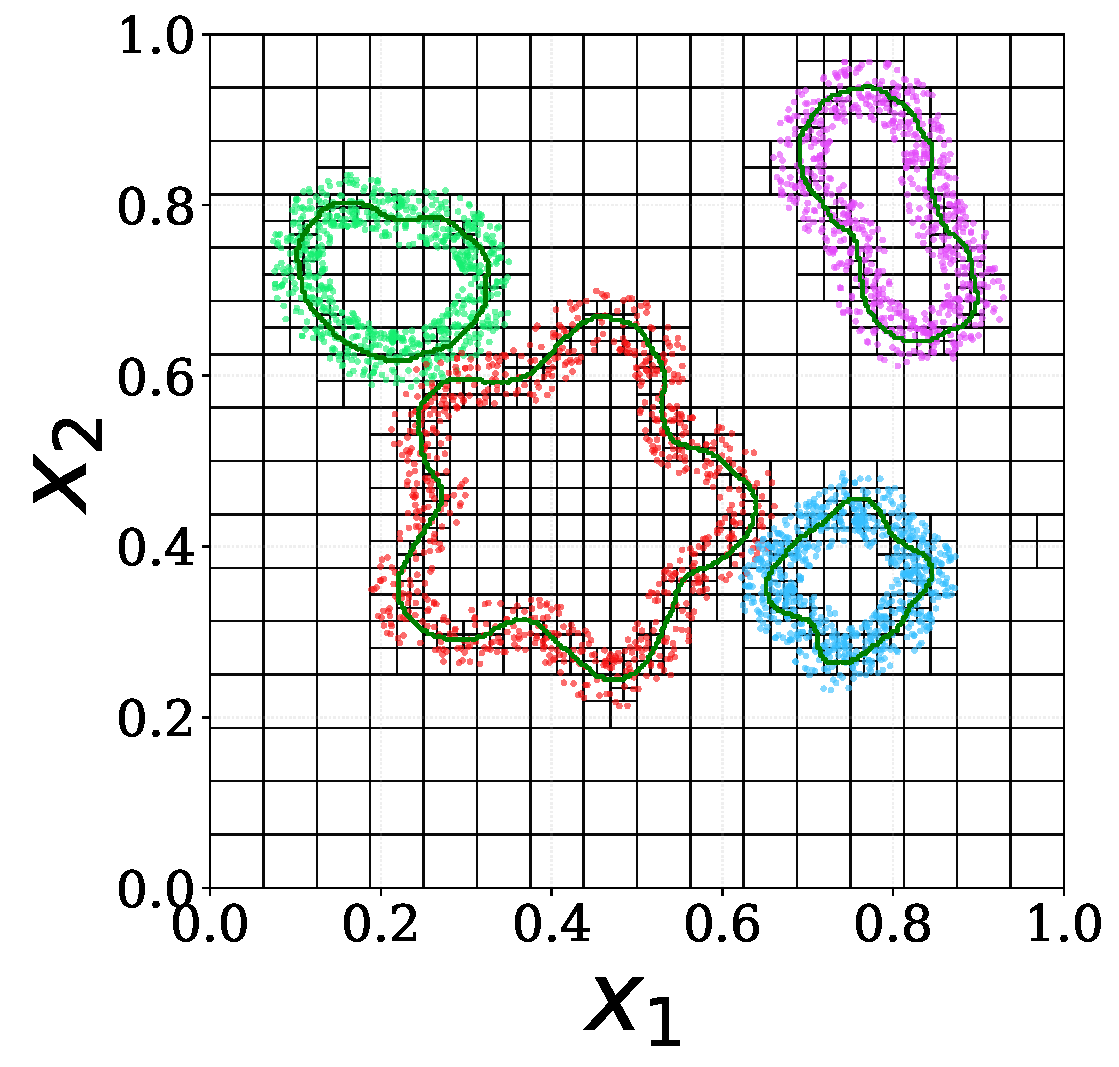
\includegraphics[width=\textwidth]{irregular_cells_and_enhance_centers.pdf}
        \caption{ $\mathcal{C}_{\text{final}}$ }
    \end{subfigure}
    \hspace{1ex}
    \begin{subfigure}[b]{0.3\textwidth}
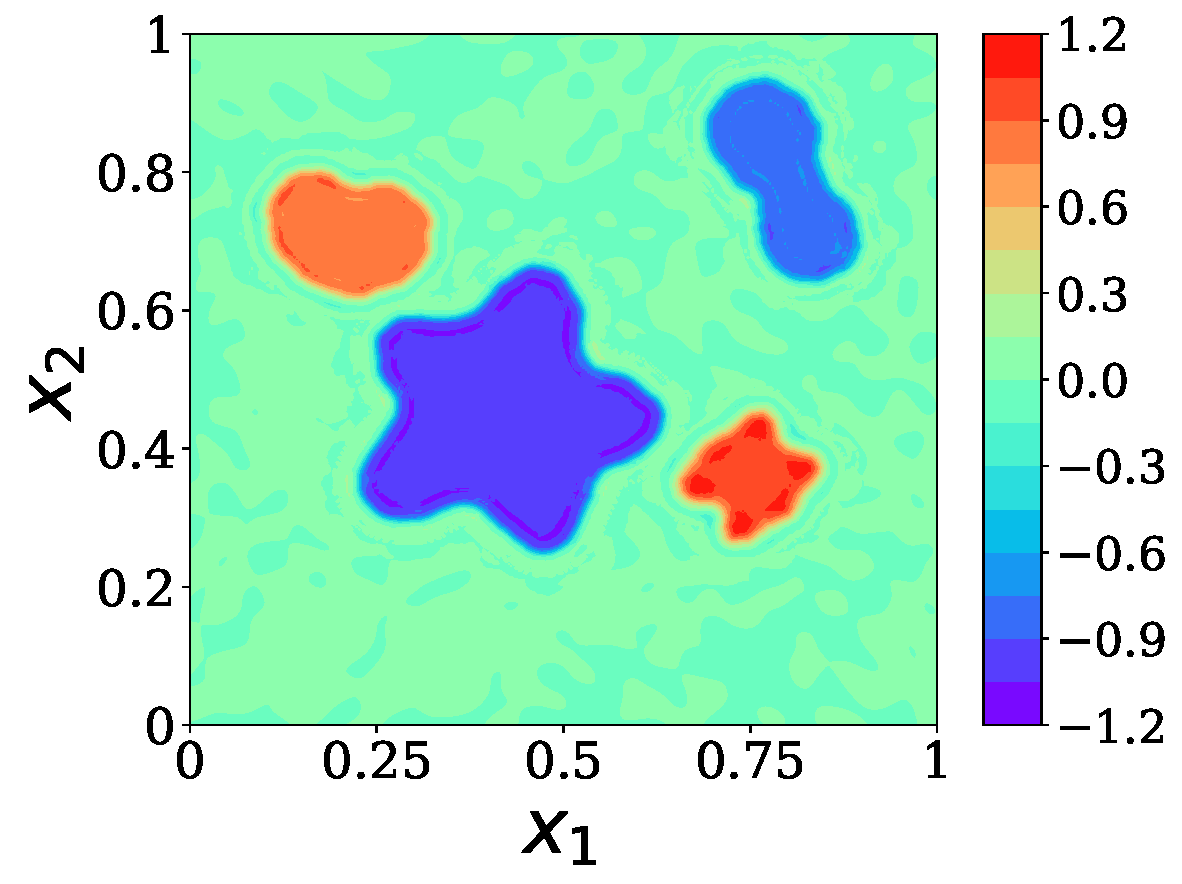
\includegraphics[width=\textwidth]{irregular_num_idx4.pdf}
        \caption{Reconstructed source}
    \end{subfigure}
    \hspace{1ex}
    \begin{subfigure}[b]{0.3\textwidth}
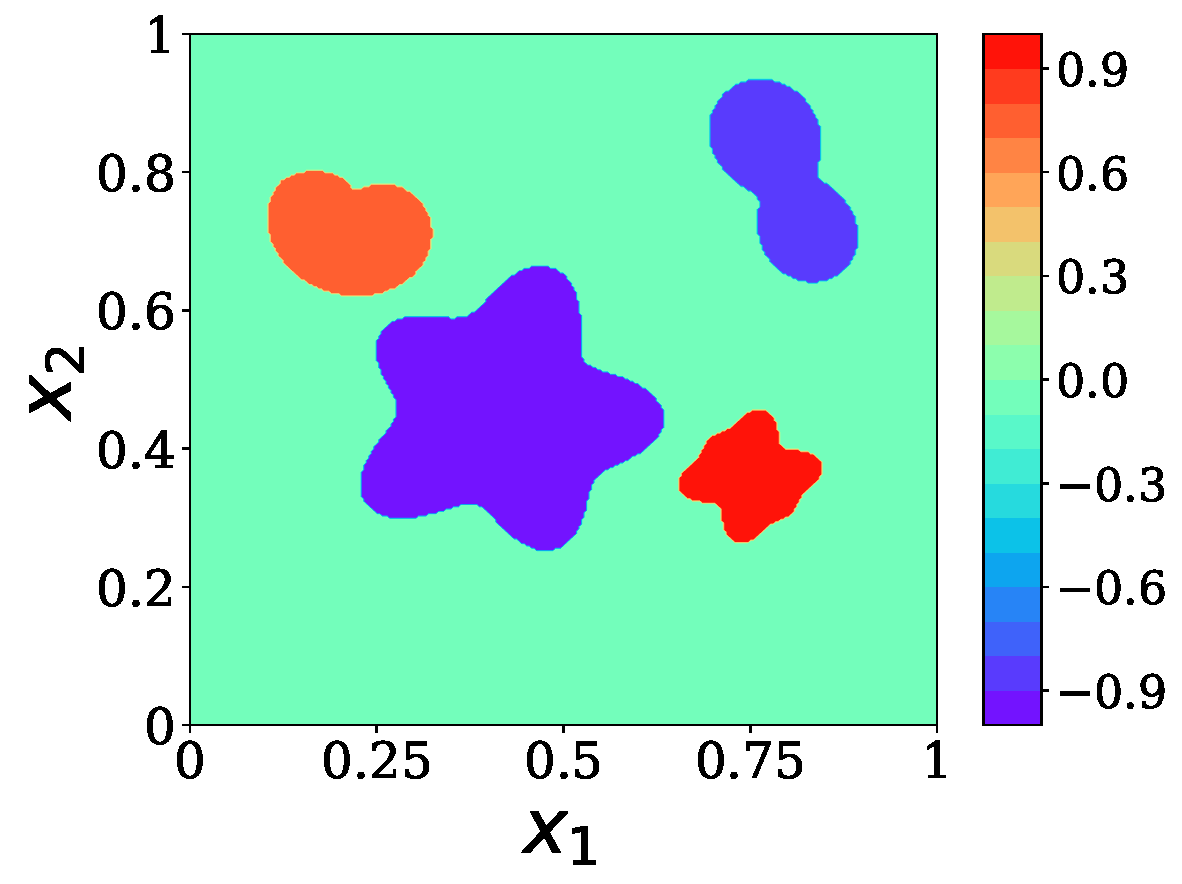
\includegraphics[width=\textwidth]{irregular_true_source.pdf}
        \caption{ {True source}}
        \label{ex:4.7:irregular}
    \end{subfigure}
    \caption{Example 4.7:\ Irregular source: (a): Final adaptive mesh ($\mathcal{C}_{\text{final}}$) obtained via IA-RFM, yielding 25.05\%, with colored circle basis centers and the nominal boundary(green solid). (b) MA-RFM results with $\delta=5\%$, $M_0=1600$, $M_{\alpha,\text{general}}=1000$, $M_{\alpha,\text{circular}}=800$, $\lambda_{\text{reg}}^2=1\times 10^{-5}$ yield $17.84\% \ E_{l^2}(S)$.}
    \label{fig:Irregular:detect_bound}
\end{figure}
In this example, Figure \ref{fig:Irregular:detect_bound} shows that the stage-one coarse reconstruction yields a relative $L^2$ error of $25.05\%$, and the final MA-RFM reconstruction achieves a relative $L^2$ error of $17.84\%$, which corresponds to an error reduction of $28.79\%$. The detected cluster patterns, morphology labels, and basis-profile choices are consistent with the true source geometry and functional form, demonstrating that Algorithm~2 can effectively drive the second-stage basis selection. The corresponding detected geometric parameters and basis-function types for this example are reported in Table~9 of the revised manuscript.}
\end{document}
